\documentclass[11pt]{article}

\usepackage[margin=1in]{geometry}
\usepackage[T1]{fontenc}
\usepackage{lmodern}
\usepackage{microtype}
\usepackage{amsmath,amssymb}
\usepackage{booktabs}
\usepackage{graphicx}
\usepackage{xcolor}
\usepackage[numbers,sort&compress]{natbib}
\usepackage[colorlinks=true,linkcolor=blue!50!black,citecolor=blue!50!black,urlcolor=blue!50!black]{hyperref}
\usepackage{caption}
\captionsetup{font=small,labelfont=bf}

\title{Who You Train Against Matters: Reward Shaping and Opponent Choice\\
for PPO in a Real-Time Two-Lane Card Battle Game}
\author{Abhay Chavda\\
\small Code and data: \url{https://github.com/Abhay-Chavda/Reinforcement_Learning_Clash_Royale}}
\date{November 2026}

\begin{document}
\maketitle

\begin{abstract}
Real-time card strategy games such as \emph{Clash Royale} combine resource
management, unit placement and continuous combat, which makes them a compact
but non-trivial testbed for reinforcement learning (RL). We build a lightweight,
open-source Gymnasium environment that captures the core loop of these games
(two lanes, three towers per side, an elixir economy and two troop types) and
use it to study two design choices that practitioners face when training a
Proximal Policy Optimization (PPO) agent: the reward signal (sparse win/loss
versus a dense damage-based shaped reward) and the training opponent (random,
rule-based heuristic, or a frozen earlier PPO agent). Across 30 training runs
(5 seeds per configuration) evaluated against three opponents, we find that
(i) against a weak random opponent both rewards work, and shaping reaches an
80\% training win rate $1.8\times$ faster; (ii) against stronger opponents the
sparse reward provides almost no learning signal (6.4\% win rate after training
against the heuristic) while shaping recovers useful policies; (iii) agents
trained only against the random opponent generalize poorly (30--32\% against
the heuristic), and the best-generalizing configuration is shaped reward
against a frozen PPO opponent (83.0\% / 55.6\% / 69.4\% against random /
heuristic / frozen-PPO opponents); and (iv) outcomes vary strongly with the
random seed (standard deviation up to 43 percentage points), so single-seed
results, which our own preliminary experiments relied on, can be misleading.
We also identify a greedy-decoding gap: shaped-reward policies win 94.2\% of
games when actions are sampled but only 69.4\% when the most likely action is
taken. All code, trained models and raw episode logs are released.
\end{abstract}

\section{Introduction}

Games have long served as benchmarks for RL, from Atari \citep{mnih2015dqn}
and Go \citep{silver2016alphago} to large real-time strategy titles such as
StarCraft~II \citep{vinyals2019alphastar} and Dota~2 \citep{berner2019dota}.
The latter results required enormous compute, which puts them out of reach for
most students and small labs. Real-time \emph{card battle} games sit between
these extremes: a match lasts a few minutes, the action space is small (which
card, which lane, when), yet good play requires managing a regenerating
resource, timing deployments, and reacting to the opponent.

This paper uses a deliberately small simulator of such a game to answer two
practical questions:

\begin{enumerate}
  \item \textbf{Reward design.} Does a dense, damage-based shaped reward help
  PPO compared with a sparse win/loss reward, and does it change
  \emph{how} the agent plays?
  \item \textbf{Opponent choice.} How does the opponent used during training
  (random, scripted heuristic, or a frozen copy of an earlier PPO agent)
  affect the strength and generality of the learned policy?
\end{enumerate}

Our contributions are:
\begin{itemize}
  \item An open-source Gymnasium \citep{towers2024gymnasium} environment for a
  two-lane, real-time card battle game with a fixed-size 149-dimensional
  observation and a mirrored opponent view, so any trained policy can be
  re-used as an opponent without modification (Section~\ref{sec:env}).
  \item A controlled study of 6 training configurations $\times$ 5 seeds,
  each evaluated on 100 held-out episodes against 3 opponents
  (Section~\ref{sec:setup}), with seed-level variability reported throughout
  as recommended by \citet{henderson2018matters} and
  \citet{agarwal2021precipice}.
  \item Behavioural analysis showing that the two reward signals produce
  qualitatively different play styles, and a greedy-decoding gap that hides
  much of the shaped agent's strength (Section~\ref{sec:results}).
\end{itemize}

\section{Related Work}

\paragraph{RL for strategy games.}
Deep RL has reached expert level in board games \citep{silver2016alphago} and
in complex real-time games \citep{vinyals2019alphastar, berner2019dota}. These
systems rely on self-play and large populations of opponents; our setting asks
the same opponent-selection question at a scale that runs on a laptop CPU.

\paragraph{Reward shaping.}
\citet{ng1999shaping} showed that shaping terms of the form
$\gamma\Phi(s') - \Phi(s)$ leave the optimal policy unchanged. Our damage term
is close to this potential-based form, but our shaped reward also includes an
invalid-action penalty that is not potential-based, and we observe that it
changes the agent's behaviour substantially (Section~\ref{sec:behaviour}).

\paragraph{Opponents and generalization.}
Training against a single fixed opponent can produce brittle strategies that
exploit that opponent; population-based and game-theoretic methods such as
PSRO \citep{lanctot2017psro} and competitive self-play
\citep{bansal2018emergent} address this. We measure the brittleness directly
by evaluating every agent against opponents it never trained against.

\paragraph{Invalid actions.}
Card games naturally have state-dependent action validity (a card cannot be
played without enough resource). \citet{huang2022masking} show that masking
invalid actions improves policy-gradient learning; here we deliberately leave
actions unmasked and study how the reward signal affects invalid-action rates.

\section{Environment}
\label{sec:env}

\paragraph{Board and towers.}
The arena is the unit square $[0,1]^2$ with two lanes at $x=0.25$ and
$x=0.75$. Each side owns two \emph{Queen} towers (2{,}500\,HP, one per lane)
and a central \emph{King} tower (5{,}000\,HP). The learning agent's towers
are at $y=0.08$ and the opponent's at $y=0.92$. Towers deal 90 damage once per
second to the nearest enemy troop within range (0.20 for Queen, 0.30 for King).

\paragraph{Troops.}
Two troop types are available (Table~\ref{tab:cards}). A troop spawns in its
lane ($y=0.15$ or $0.85$), engages the nearest enemy troop in the same lane,
and otherwise walks to the enemy Queen tower of its lane, then to the King
tower once that Queen tower is destroyed.

\begin{table}[h]
\centering
\small
\begin{tabular}{lcccccc}
\toprule
Card & Elixir & HP & Damage & Speed & Range & Attack cooldown (s) \\
\midrule
Knight & 3 & 1000 & 100 & 0.20 & 0.05 & 1.0 \\
Giant  & 5 & 2000 & 200 & 0.10 & 0.05 & 1.5 \\
\bottomrule
\end{tabular}
\caption{Troop statistics. Distances are in board units, speed in units per second.}
\label{tab:cards}
\end{table}

\paragraph{Economy and timing.}
Both players start with 5 elixir, regenerate 0.5 elixir per second, and are
capped at 10. The simulation advances in steps of $\Delta t = 0.5$\,s and a
match lasts 120\,s (240 agent decisions). The opponent acts once per second.

\paragraph{Actions.}
The action space is $\mathcal{A}=\{$wait, Knight-left, Knight-right,
Giant-left, Giant-right$\}$. Choosing a card without enough elixir is an
\emph{invalid action}: nothing is deployed and the step continues.

\paragraph{Observations.}
The 149-dimensional observation, normalized to $[0,1]$, contains 9 global
features (own and enemy tower HP, own and enemy elixir, time remaining) and
10 fixed slots per side for troops, each with 7 features (active flag, troop
type, lane, $x$, $y$, HP fraction, attack-cooldown fraction).
For an opponent policy the environment builds the same vector from the other
side's perspective: the sides are swapped and every $y$ coordinate is mapped
to $1-y$. Because the board is symmetric under this reflection and lanes keep
their $x$ position, a policy trained as the bottom player can control the top
player unchanged.\footnote{An earlier version of our code passed the
\emph{player's} observation to the frozen opponent, so it acted on a flipped
board. Results in this paper use the corrected, mirrored view; unit tests
check the mirroring.}

\paragraph{Termination and outcome.}
A match ends immediately when a King tower is destroyed. Otherwise, at
time-out the side with more total tower HP wins; equal HP is a draw.

\paragraph{Rewards.}
The \emph{sparse} reward is $+1$ for a win, $-1$ for a loss and $0$ otherwise,
given only at the final step. The \emph{shaped} reward adds, at every step,
\begin{equation}
  r^{\text{shape}}_t = 0.0002\,\big(D^{\text{dealt}}_t - D^{\text{taken}}_t\big)
  - 0.01\cdot\mathbb{1}[\text{action $t$ invalid}],
\end{equation}
where $D_t$ is the tower damage dealt or taken during the step. Since all
towers together hold 10{,}000\,HP, the damage term is bounded by $\pm 2$ per
episode, the same order as the terminal reward.

\section{Experimental Setup}
\label{sec:setup}

\paragraph{Agent.}
We use PPO \citep{schulman2017ppo} with generalized advantage estimation
\citep{schulman2016gae} from Stable-Baselines3 \citep{raffin2021sb3}, with the
default MLP policy (two hidden layers of 64 units for actor and critic) and
hyperparameters: learning rate $3\cdot10^{-4}$, $n_\text{steps}=1024$, batch
size 64, 10 epochs, $\gamma=0.99$, $\lambda_\text{GAE}=0.95$, clip range 0.2,
entropy coefficient 0.01. Each run trains for 100{,}000 environment steps
(about 420 matches) on CPU.

\paragraph{Training opponents.}
\begin{itemize}
  \item \textbf{Random}: every second, chooses uniformly among affordable actions (including wait).
  \item \textbf{Heuristic}: a hand-written ``defend, then push'' rule: if an
  enemy troop is in its half of a lane, deploy a Knight there; otherwise save
  to 8 elixir and send a Giant to the lane whose enemy Queen tower is weaker.
  \item \textbf{Frozen PPO}: the sparse-reward agent trained against the
  random opponent with seed 7, used with greedy actions and the mirrored
  observation.
\end{itemize}

\paragraph{Configurations.}
We cross the two rewards with the three training opponents (6 configurations)
and train each with seeds $\{7, 42, 123, 2024, 31337\}$, for 30 runs in total.
We label configurations as \emph{Reward $|$ Opponent}, e.g.\ \emph{Shaped
$|$ PPO}. A random agent and the heuristic, used as the learning side, serve
as non-learning baselines.

\paragraph{Evaluation protocol.}
Every agent plays 100 matches against each of the three opponents, using
environment seeds 1000--1099, which are never used in training. PPO agents act
greedily (most likely action) unless stated otherwise. The heuristic and
frozen-PPO opponents are deterministic, and so is the simulator, so without
intervention all 100 matches against them would be the same game; during
evaluation they therefore replace each decision with a random affordable
action with probability $\varepsilon=0.1$, seeded per match. We report the
mean and standard deviation of the win rate across the 5 seeds, and 95\%
Wilson intervals \citep{wilson1927} for the 500 pooled matches.

\section{Results}
\label{sec:results}

\begin{table}[t]
\centering
\small
\begin{tabular}{lccc}
\toprule
Agent (reward $|$ training opponent) & Random & Heuristic & Frozen-PPO \\
\midrule
Random & 29.0 & 0.0 & 5.0 \\
Heuristic & 95.0 & 19.0 & 25.0 \\
\midrule
Sparse $|$ Rand & \textbf{88.2 $\pm$ 11.5} & 30.0 $\pm$ 7.8 & 61.4 $\pm$ 19.9 \\
Shaped $|$ Rand & 69.4 $\pm$ 10.5 & 31.8 $\pm$ 32.2 & 33.8 $\pm$ 22.6 \\
Sparse $|$ Heur & 48.2 $\pm$ 30.7 & 6.4 $\pm$ 11.1 & 28.0 $\pm$ 36.6 \\
Shaped $|$ Heur & 61.8 $\pm$ 28.7 & 34.4 $\pm$ 35.9 & 56.8 $\pm$ 36.2 \\
Sparse $|$ PPO & 81.8 $\pm$ 9.7 & 32.0 $\pm$ 43.4 & 46.2 $\pm$ 32.5 \\
Shaped $|$ PPO & 83.0 $\pm$ 19.0 & \textbf{55.6 $\pm$ 42.9} & \textbf{69.4 $\pm$ 36.3} \\
\bottomrule
\end{tabular}

\caption{Evaluation win rate (\%) against each opponent: mean $\pm$ standard
deviation over 5 training seeds, 100 matches per seed. Bold marks the best PPO
configuration per column. Baselines are single agents.}
\label{tab:main}
\end{table}

\begin{figure}[t]
\centering
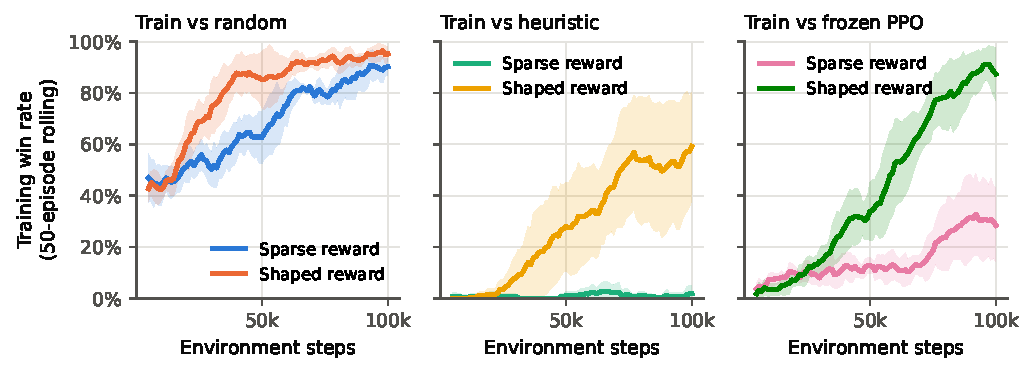
\includegraphics[width=\linewidth]{figures/learning_curves.pdf}
\caption{Training win rate (50-episode rolling mean; line = mean over 5 seeds,
band = $\pm 1$ s.d.) for each training opponent. With the sparse reward, PPO
barely learns against the heuristic and learns slowly against the frozen PPO
opponent.}
\label{fig:curves}
\end{figure}

\begin{figure}[t]
\centering
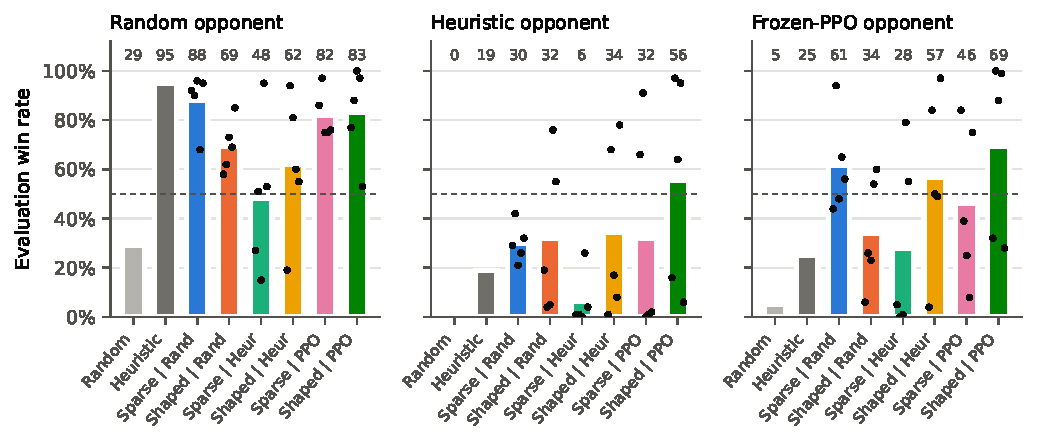
\includegraphics[width=\linewidth]{figures/eval_win_rates.pdf}
\caption{Evaluation win rate per configuration and opponent. Bars show the
mean over seeds (value printed above); dots are individual seeds. The dashed
line marks 50\%.}
\label{fig:eval}
\end{figure}

\subsection{Against a weak opponent, both rewards work; shaping learns faster}

Against the random opponent, all PPO configurations clearly beat the random
baseline (29.0\%). Training curves (Figure~\ref{fig:curves}, left) show that
the shaped reward reaches an 80\% rolling training win rate after
33.6k steps on average versus 59.9k for the sparse reward, a $1.8\times$
speed-up. In greedy evaluation, however, \emph{Sparse $|$ Rand} scores higher
(88.2\% vs.\ 69.4\%, Table~\ref{tab:main}). Section~\ref{sec:greedy} shows
that this reversal comes from greedy action selection, not from a weaker policy.

The scripted heuristic is a strong baseline against random play (95.0\%), but
it mostly wins on tower HP at time-out and never destroys a King tower
(Table~\ref{tab:detail}).

\subsection{Against stronger opponents, the sparse reward stops working}

When the training opponent is the heuristic, sparse-reward PPO almost never
wins a training match (Figure~\ref{fig:curves}, middle) and therefore gets
almost no positive signal: its training win rate stays near 0\% and its
evaluation win rate against the heuristic is 6.4\%. With shaping, every match
still produces graded feedback through tower damage, and the training win
rate climbs to about 60\%. The same pattern, less extreme, appears against the
frozen PPO opponent (about 30\% vs.\ 87\% final training win rate). In short,
shaping matters most exactly when wins are rare.

\subsection{Generalization depends on the training opponent}

Agents trained only against the random opponent transfer poorly: both
\emph{Sparse $|$ Rand} and \emph{Shaped $|$ Rand} win only 30--32\% against the
heuristic. The best overall configuration is \emph{Shaped $|$ PPO}, which
achieves 83.0\% against random, 55.6\% against the heuristic (the heuristic itself wins only 19.0\% of
this match-up) and 69.4\% against the frozen PPO
agent. Training against a competent learned opponent therefore produced more
general play than training against either a random or a scripted opponent,
consistent with the motivation for self-play and opponent populations
\citep{bansal2018emergent, lanctot2017psro}.

\subsection{Seed variance is large}

The dots in Figure~\ref{fig:eval} show that individual seeds of the same
configuration can range from near 0\% to above 90\% against the same opponent
(e.g.\ \emph{Shaped $|$ PPO} vs.\ heuristic: 6\%, 16\%, 64\%, 95\%, 97\%).
Our preliminary single-seed experiments reported win rates between 69\% and
100\% for individual seeds; these were real for those seeds but overstated what a
configuration reliably achieves. This mirrors the reproducibility concerns of
\citet{henderson2018matters}, and all conclusions above are based on the
5-seed means, the pooled confidence intervals in Table~\ref{tab:detail}, and
patterns that hold across seeds.

\subsection{The two rewards produce different play styles}
\label{sec:behaviour}

\begin{table}[t]
\centering
\small
\begin{tabular}{lccccc}
\toprule
Agent & W / D / L & 95\% CI (pooled) & King kills & HP margin & Invalid \\
\midrule
Random & 29 / 3 / 68 & [21.0, 38.5] & 0\% & -489 & 0.0\% \\
Heuristic & 95 / 1 / 4 & [88.8, 97.8] & 0\% & +2094 & 0.0\% \\
Sparse $|$ Rand & 441 / 7 / 52 & [85.1, 90.7] & 7\% & +1944 & 78.9\% \\
Shaped $|$ Rand & 347 / 9 / 144 & [65.2, 73.3] & 32\% & +1092 & 9.0\% \\
Sparse $|$ Heur & 241 / 2 / 257 & [43.9, 52.6] & 26\% & -454 & 84.6\% \\
Shaped $|$ Heur & 309 / 2 / 189 & [57.5, 66.0] & 59\% & +148 & 21.8\% \\
Sparse $|$ PPO & 409 / 9 / 82 & [78.2, 84.9] & 18\% & +2149 & 73.7\% \\
Shaped $|$ PPO & 415 / 1 / 84 & [79.5, 86.0] & 62\% & +3042 & 23.7\% \\
\bottomrule
\end{tabular}

\caption{Detailed outcomes against the random opponent (500 pooled matches per
PPO configuration, 100 per baseline). \emph{King kills}: share of wins that
ended by destroying the King tower rather than at time-out. \emph{HP margin}:
mean own minus enemy total tower HP at the end. \emph{Invalid}: share of
decisions that tried to play an unaffordable card.}
\label{tab:detail}
\end{table}

\begin{figure}[t]
\centering
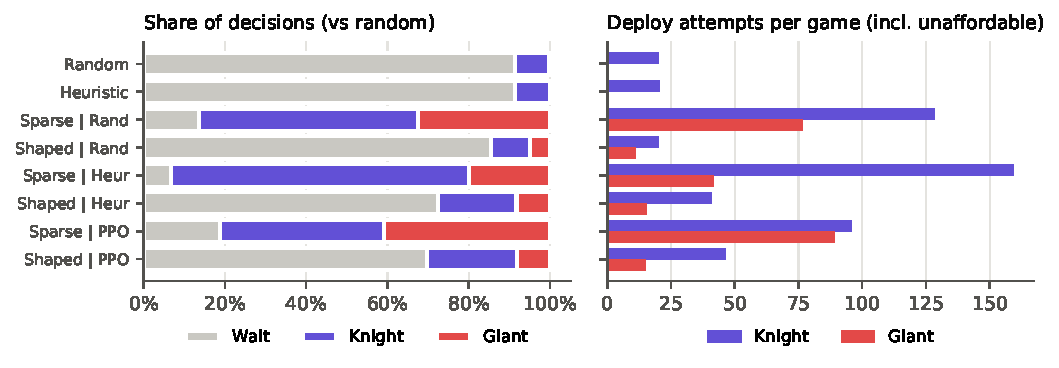
\includegraphics[width=\linewidth]{figures/action_distribution.pdf}
\caption{Action usage against the random opponent. Left: share of the 240
decisions per match. Right: deployment attempts per match, including
unaffordable ones.}
\label{fig:actions}
\end{figure}

Figure~\ref{fig:actions} and Table~\ref{tab:detail} show a sharp behavioural
difference. Sparse-reward agents almost never choose \emph{wait} (7--19\% of
decisions) and attempt to deploy a card on nearly every step, so 74--85\% of
their decisions are invalid. Because an invalid action costs nothing under the
sparse reward, this ``always press a card'' policy is a simple way to deploy
as soon as elixir allows. These agents mostly win on HP at time-out (King kills
in only 7--26\% of wins).

Shaped-reward agents, penalized $-0.01$ per invalid action, wait for 69--85\%
of decisions and cut the invalid rate to 9--24\%. They also play more
decisively: 32--62\% of their wins destroy the King tower, and matches end
earlier (195--223 steps on average vs.\ 217--234). The invalid-action penalty
is not potential-based \citep{ng1999shaping}, so it is expected to change the
optimal policy, and it does.

\subsection{Greedy decoding hides the shaped agent's strength}
\label{sec:greedy}

\begin{table}[t]
\centering
\small
\begin{tabular}{llcc}
\toprule
Reward & Action selection & Win rate vs.\ random (\%) & Wait share (\%) \\
\midrule
Sparse & Greedy  & 88.2 $\pm$ 11.5 & 13.3 \\
Sparse & Sampled & 89.4 $\pm$ \phantom{0}3.4 & 14.0 \\
Shaped & Greedy  & 69.4 $\pm$ 10.5 & 85.5 \\
Shaped & Sampled & \textbf{94.2 $\pm$ \phantom{0}3.3} & 72.3 \\
\bottomrule
\end{tabular}
\caption{Greedy (most likely action) vs.\ sampled actions for agents trained
against the random opponent (5 seeds, 100 matches each).}
\label{tab:greedy}
\end{table}

The shaped agents' training win rate (about 95\%, Figure~\ref{fig:curves})
is far higher than their greedy evaluation win rate (69.4\%). Since training
uses sampled actions, we re-evaluated the agents trained against the random
opponent with sampled actions (Table~\ref{tab:greedy}). Sampling raises the
shaped agents to 94.2\%, the best result against the random opponent in this
study, and also reduces the seed spread, while the sparse agents barely
change. Our interpretation is that the shaped policy keeps \emph{wait} as the
single most likely action in most states and deploys through the remaining
probability mass; taking the most likely action every time collapses this
into excessive waiting (85.5\% of decisions). Practitioners should therefore
check both action-selection modes before comparing reward designs.

\section{Limitations}

\begin{itemize}
  \item \textbf{Simplified game.} Two troop types, no spells, no buildings,
  no card cycle or hand, and no air units. Giants, for example, engage troops
  in our simulator rather than targeting only buildings.
  \item \textbf{Asymmetric timing.} The learning agent decides every 0.5\,s and
  the opponent every 1\,s, and the agent's troops are updated first within
  a step. Mirror matches are therefore not exactly 50/50 (e.g.\ random vs.\
  random: 29\%; heuristic vs.\ $\varepsilon$-heuristic: 19\%), and win rates
  should be compared across agents rather than read as absolute strength.
  \item \textbf{Scale.} 100k steps per run and 5 seeds; longer training,
  hyperparameter tuning and more seeds may change the ranking of close
  configurations.
  \item \textbf{Single frozen opponent.} We use one fixed PPO opponent rather
  than iterated self-play or a population.
  \item \textbf{Evaluation noise.} The $\varepsilon=0.1$ perturbation makes the
  heuristic and frozen-PPO opponents slightly weaker than in training.
\end{itemize}

\section{Conclusion and Future Work}

In a small real-time card battle game, the choice of training opponent and
reward signal changes both how strong a PPO agent becomes and how it plays.
Shaped rewards matter most when the opponent is strong enough that wins are
rare; training against a frozen learned opponent with a shaped reward gave
the most general agents; and both seed variance and greedy decoding can
change the apparent ranking of methods. Natural next steps are invalid-action
masking \citep{huang2022masking}, iterated self-play with an opponent pool,
richer card sets with a hand-and-cycle mechanic, and a symmetric decision
schedule for both players.

\paragraph{Reproducibility.}
\texttt{run\_all.sh} retrains all 30 agents and regenerates every table and
figure (about 35 minutes on a 16-thread CPU). The repository includes trained
models, TensorBoard logs, per-episode training logs and all 9{,}600 evaluation
episodes as CSV files.

\bibliographystyle{plainnat}
\bibliography{references}

\end{document}
